\documentclass[11pt]{article}

\usepackage{graphicx}
\usepackage{amssymb,amsmath}

\newcommand\amtx{\boldsymbol{A}}
\newcommand\bmtx{\boldsymbol{B}}

\newcommand\xmtx{\boldsymbol{X}}
\newcommand\betavec{\boldsymbol{\beta}}

\newcommand\yvec{\boldsymbol{y}}
\newcommand\yhat{\hat{y}}
\newcommand\yhatvec{\boldsymbol{\hat{y}}}

\title{Linear regression notes}
\author{John Bogovic}
\date{2019 July}

\begin{document}

\maketitle

\section{ Review }

To be multiplied, matrices need to have the same ``inner'' dimensions:
the number of columns of the left matrix must equal the number of rows
of the right matrix.
\begin{equation}
    \amtx_{L \times M } \bmtx_{M \times N} = \xmtx_{L \times N }
\end{equation}

but 
\begin{equation}
    \amtx_{L \times M } \bmtx_{N \times M} = \mathrm{ nothing, nonsense }
\end{equation}

This works:
\begin{equation}
    \amtx_{L \times M } \bmtx_{N \times M}^T =  \xmtx_{L \times N }
\end{equation}

\subsection{ Exercise }

If $\amtx_{M \times N}$, what size is $A^T A$?
\begin{enumerate}
    \item $N \times N$
    \item $M \times N$
    \item $M \times M$
    \item Stupid question, because you can't multiply them.
\end{enumerate}





\section{ Simple linear regression (fit a 1d line)}

\subsection{The problem}

We are given the value of a variable, $x$, we would like to predict
the value of another variable $y$.  You will often see $x$ called the
``independent variable'', and $y$ called the ``dependent variable''.
We have many pairs of observations:
\begin{equation}
    \begin{array}{l}
    x_1, y_1 \\
    x_2, y_2 \\
    \vdots \\
    x_N, y_N \\
    \end{array}
\end{equation}


Linear regression (1d) does this by finding the linear function that
gives the best predictions.  The functions we have to consider are:

\begin{equation}
    \hat{y} = ax + b
\end{equation}

Where we wrote $\hat{y}$ instead of $y$ to indicate that it is an
estimate, or prediction, and not the true value of $y$ for the given
$x$. Another way to think of the task is that we need to  find the
values $a$ and $b$ that give us the best results. The values $a$ and $b$
are called ``parameters'' of the function.  How do we measure how good
the predictions are?

\subsection{``Cost function'' - measuring goodness of the prediction}

The most common way is to use the ``sum of squared differences'' (SSD) also
called ``sum of squared errors'' (SSE), or``residual sum of squares.''
It is computed like this:

\begin{equation}
    SSD(a,b) = \sum_i (y_i - (ax_i + b))^2.
\end{equation}

Notice that $ax_i +b$ is the value of $y$ predicted by our function for the
input $x_i$.  This is an \emph{``ordinary'' linear least squares} problem.
Figure \ref{fig:ssd} shows a visualization of SSD. 

\begin{figure}[h]
    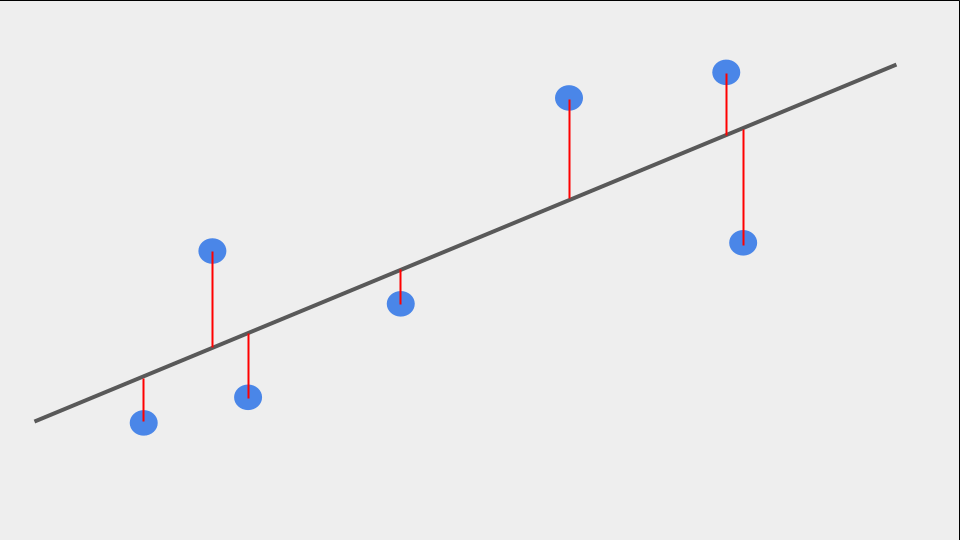
\includegraphics[width=0.7\textwidth]{SSD.png}
    \centering
    \caption{Adding the (squared) lengths of the red lines will tell us
    how good this fit is.  Notice that the distances we sum are
    \emph{not} the shorted lines from the point to the line, but rather
    the vertical distance to the line. }
    \label{fig:ssd}
\end{figure}

A related measure, the Root mean squared error (RMSE) is:
\begin{equation}
    RMSE = \sqrt{\frac{SSD}{N}}
\end{equation}
where $N$ is the number of data points.
Yet another measure is $R^2$ (``R-squared''), which compares the linear
model to a ``baseline'' model which always predicts the same value (the
mean of our observations: $\bar{y}$) for $y$, regardless of what $x$ is.  

\begin{equation}
    R^2 = 
        1 - \frac{ \sum_i (y_i - \hat{y}_i)^2 }{ \sum (y_i - \hat{y}_i)^2} = 
        1 - \frac{ SSD }{ SST }
\end{equation}

where SST is the ``total sum of squares''


\subsection{Rewrite the problem using linear algebra}

It might seem strange to do this now, but it will help us find a solution
to the problem and help us use the technique when we have many input
and/or output variables.

The linear function that does the prediction is:
\begin{equation}
    \begin{bmatrix}
        \yhat
    \end{bmatrix}
    = 
    \begin{bmatrix}
        1 & x 
    \end{bmatrix}
    \begin{bmatrix}
        b \\ a
    \end{bmatrix}
\end{equation}

To determine the parameters $a$ and $b$, we need to consider all the
pairs of data points at once. We have as many equations as we have data
point pairs ($N$).  First, let's stack the $y_i$ in a vector.
\begin{equation}
    \begin{bmatrix}
        y_1  \\
        y_2 \\
        \vdots \\
        y_N
    \end{bmatrix}
\end{equation}

Next, observe that we can write the vector of function predictions like this:

\begin{equation}
    \begin{bmatrix}
        y_1 \\
        y_2 \\
        \vdots \\
        y_N
    \end{bmatrix}
    \approx 
    \begin{bmatrix}
        \yhat_1 \\
        \yhat_2 \\
        \vdots \\
        \yhat_N
    \end{bmatrix}
    =
    \begin{bmatrix}
        x_1 & 1 \\
        x_2 & 1 \\
        \vdots \\
        x_N & 1
    \end{bmatrix}
    \begin{bmatrix}
        a \\ b
    \end{bmatrix}
\end{equation}

Let's give names to the vectors and matrices:
\begin{equation}
    \yvec \approx \yhatvec = \xmtx \betavec
\end{equation}

Remember, at this point we have values for the $x_i$ and $y_i$ (the
$\xmtx$ matrix and the $\yvec$ vector). We need to find the best values
for $a$ and $b$ (the $\betavec$ vector).

\subsection{Finding the solution}

We can use our linear algebra to find the solution. One way is using the normal equations:
\begin{equation}
    \betavec = (\xmtx^T \xmtx)^{-1} \xmtx^T \yvec
\end{equation}

where does this come from?

\begin{equation}
    \begin{aligned}
        C &= ( \yvec - \yhatvec )^T( \yvec - \yhatvec ) \\
          &= ( \yvec - \xmtx \betavec )^T( \yvec - \xmtx\betavec ) \\
          &= \yvec^T \yvec  - \yvec^T \xmtx \betavec - \betavec^T \xmtx^T \yvec + 
                \betavec^T \xmtx^T \xmtx \betavec \\
          &= \yvec^T \yvec  - 2 \yvec^T \xmtx \betavec + \betavec^T \xmtx^T \xmtx \betavec 
    \end{aligned}
\end{equation}

Now take the derivative:
\begin{equation}
    \begin{aligned}
        \frac{dC}{d\betavec} &= \frac{d}{d\betavec} 
            (\yvec^T \yvec  - 2 \yvec^T \xmtx \betavec + \betavec^T \xmtx^T \xmtx \betavec )\\
            &= (- 2 \yvec^T \xmtx + 2 \xmtx^T \xmtx \betavec )\\
    \end{aligned}
\end{equation}

Set it equal to zero and solve for $\betavec$:
\begin{equation}
    \begin{aligned}
        0 &= (- 2 \yvec^T \xmtx + 2 \xmtx^T \xmtx \betavec ) \\
          &= -\yvec^T \xmtx + \xmtx^T \xmtx \betavec \\
         \yvec^T \xmtx &=  \xmtx^T \xmtx \betavec \\
    \end{aligned}
\end{equation}



\subsection{ Exercise }

We can't use the inverse of $\xmtx$ to solve for the best parameters.
Three of the statements below give correct reasons for why, which one is
wrong?

\begin{enumerate}
    \item $\xmtx$ is not square.
    \item There might not exist parameters that solve the equation
        $\yvec = \xmtx \betavec$
    \item The task is to find the best approximation, not to find an
        exact answer.
    \item THE WRONG ANSWER
\end{enumerate}

\section{ Multi-variable linear regression }

Now that we know how to write the linear regression problem as a matrix
equation, it is relatively straightforward to extend it to the
multi-variable case. In this set-up, we have several dependent variables to
predict, and also have several independent variables to predict them
from.

Suppose we want to predict two variables from two other variables.
Say the two things we want to predict are:
\begin{enumerate}
    \item $y_1$: the price of eggs in one months
    \item $y_2$: the price of eggs in one year
\end{enumerate}
and the two variables we can measure are:
\begin{enumerate}
    \item $x_1$: the price of eggs today
    \item $x_2$: the price of milk today
\end{enumerate}

The equations will then look like:
\begin{equation}
    \begin{array}{l}
    \yhat_1 = \alpha_0 + \alpha_1 x_1  + \alpha_2 x_2 \\
    \yhat_2 = \beta_0 + \beta_1 x_1  + \beta_2 x_2 \\
    \end{array}
\end{equation}

We can write this system of equations with matrices like this:
\begin{equation}
    \begin{bmatrix}
        \yhat_1 & \yhat_2
    \end{bmatrix} = 
    \begin{bmatrix}
        1 & x_1 & x_2 \\
    \end{bmatrix}
    \begin{bmatrix}
        \alpha_0 & \beta_0 \\
        \alpha_1 & \beta_1 \\
        \alpha_2 & \beta_2 \\
    \end{bmatrix}
\end{equation}

%\begin{equation}
%    \yhatvect = 
%    \begin{bmatrix}
%        y_1 \\ y_2
%    \end{bmatrix}  
%\end{equation}



\subsection{ Exercise }

Suppose we need to predict two output variables from three input
variables, with an offset.  What size will the matrix $\xmtx$ be?
\begin{enumerate}
    \item $3 \times 2$
    \item $2 \times 3$
    \item $4 \times 3$
    \item $3 \times 4$
\end{enumerate}


%\section{ Polynomial regression }

%\section{ General regression }


\end{document}
